\chapter{Array Architecture}

In this chapter, we first look at how localization accuracy is affected by TDOA accuracy in a two microphone setup. We then explore different microphone array configurations and select one that gives a good localization accuracy while being portable.

\section{Two Microphones}
As was mentioned in the previous chapter, points with the same TDOA to two fixed locations form a hyperbola on a 2D plane. However, in practical systems we can only measure TDOA up to a precision. Therefore we look at all points with difference of distance close to some target value within measurement error $\epsilon$. This $\epsilon$ represents accuracy on the measurement of difference of distances, and in practice it is related to sampling rate and estimation techniques. In this chapter we evaluate the impact of difference of distance estimation on localization accuracy.

\begin{figure}[]
  \centering
  \begin{subfigure}[]{.48\textwidth}
    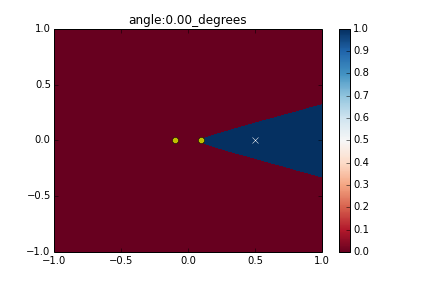
\includegraphics[width=\textwidth]{sim/sim_2_1}
    \caption{source at $(r=50$ cm, $\theta = 0$ degrees$)$}
  \end{subfigure}
  \begin{subfigure}[]{.48\textwidth}
    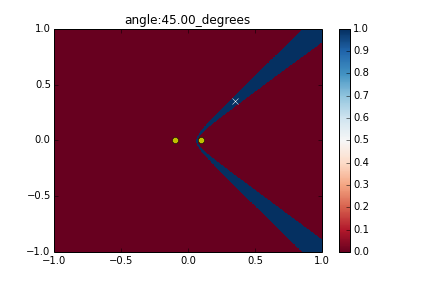
\includegraphics[width=\textwidth]{sim/sim_2_2}
    \caption{source at $(r=50$ cm, $\theta = 45$ degrees$)$}
  \end{subfigure}
%  \begin{subfigure}[]{.3\textwidth}
%    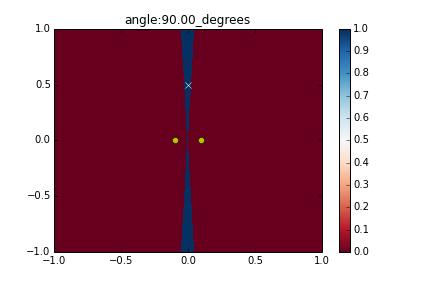
\includegraphics[width=\textwidth]{sim/sim_2_3}
%    \caption{source at $(r=50$ cm, $\theta = 90$ degrees$)$}
%  \end{subfigure}
  \caption{Uncertainty region. Yellow dots represent microphones' locations and the white dot represents the location of the source.}
  \label{fig:sim_2_5}
\end{figure}

To see how precision affects localization accuracy, we simulated two microphones placed at: $M_1:(x=-10\mbox{ cm},y=0\mbox{ cm})$ and $M_2:(x=10\mbox{ cm},y=0\mbox{ cm})$. A test sound source is emitted at point $P$ which is $50$ centimeters away from the origin $(0,0)$. Let $2a$ denote the TDOA between $P$ and two microphones:
\[
2a = \frac{P M_1 - P M_2}{340\mbox{ m/s}}
\]
where $340$ m/s is used as the speed of sound. Assuming a sampling rate of $34$ KHz, fig~\ref{fig:sim_2_5} shows the region $R$ where all points have TDOA close to $2a$ s within one sample difference:
\[
R=\{\hat P: |\frac{(\hat P M_1 - \hat P M_2)}{340\mbox{ m/s}} - 2a|< \frac{1}{2} \mbox{ samples}\}
\]
Intuitively, points in $R$ have TDOA to two microphones very similar to each other. Looking at fig~\ref{fig:sim_2_5}, we can still see that $R$ has the shape of a hyperbola, but with an uncertainty region around it. The thickness of the uncertainty region is not uniform around the hyperbola, the farther away the point is, the larger the uncertainty region becomes. This indicates for the same delta distance movement it will generate smaller TDOA change when the source is farther away from the array. The size of the uncertainty region is also angle dependent: points closer to the line connecting microphones have larger region compared to points close to the line bisecting microphones. 

This can also be seen analytically. Assuming two microphones are placed on the x-axis at $M_1:(-c,0)$ and $M2:(c,0)$. All points $P:(x,y)$ with difference of distance $ |PM_1 - PM_2| = 2a$ satisfies:
\begin{eqnarray}\label{eqn:hyperbola}
\frac{x^2}{a^2} - \frac{y^2}{c^2-a^2} = 1
\end{eqnarray}
To see how the difference of distance changes with respect to source location, we can expand the equation and find the partial differential $\frac{\partial a}{\partial x}$:
\begin{eqnarray}\label{eqn:derivative}
\frac{\partial a}{\partial x} = \frac{x(c^2-a^2)}{a(x^2+y^2+c^2)-2a^3}
\end{eqnarray}
Since all points in equation~\ref{eqn:derivative} must lie on the hyperbola, we can substitute~\ref{eqn:hyperbola} into~\ref{eqn:derivative}:
\begin{eqnarray}\label{eqn:derivativeF}
\frac{\partial a}{\partial x} = \frac{c^2-a^2}{\frac{c^2}{a}x - \frac{a^3}{x}}
\end{eqnarray}

The denominator of equation~\ref{eqn:derivativeF} increases monotonically as $|x|$ increases, which indicates $\frac{\partial a}{\partial x}$ decreases as we move farther away along the hyperbola. The same distance move $\delta x$ would generate smaller change in difference of distance $a$ when the source is farther away from the microphones. 

\begin{figure*}[]
  \centering
  \begin{subfigure}[]{.48\textwidth}
    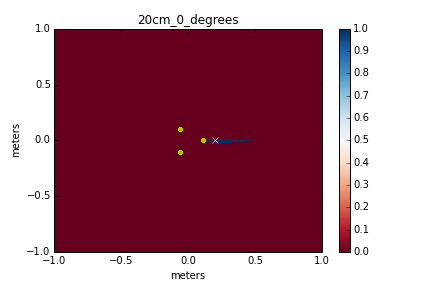
\includegraphics[width=\textwidth]{sim/result_20cm_0_degrees}
    \caption{0 degrees}
  \end{subfigure}
%  \begin{subfigure}[]{.3\textwidth}
%    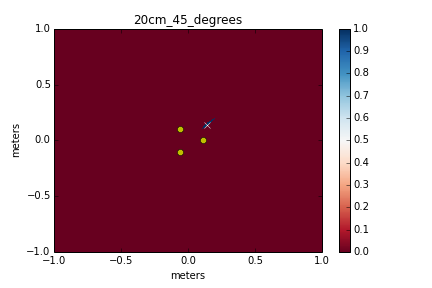
\includegraphics[width=\textwidth]{sim/result_20cm_45_degrees}
%    \caption{45 degrees}
%  \end{subfigure}
%  \begin{subfigure}[]{.3\textwidth}
%    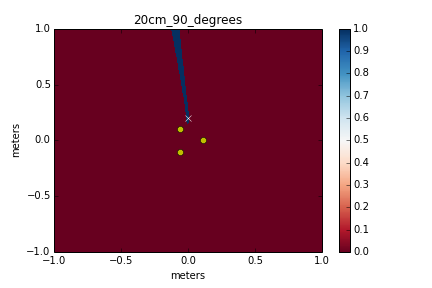
\includegraphics[width=\textwidth]{sim/result_20cm_90_degrees}
%    \caption{90 degrees}
%  \end{subfigure}
  \begin{subfigure}[]{.48\textwidth}
    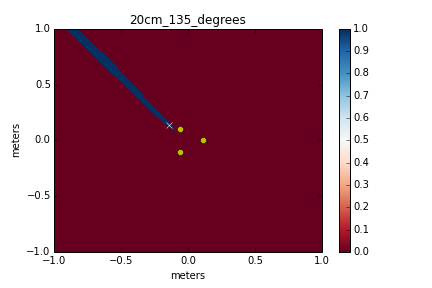
\includegraphics[width=\textwidth]{sim/result_20cm_135_degrees}
    \caption{135 degrees}
  \end{subfigure}
%  \begin{subfigure}[]{.3\textwidth}
%    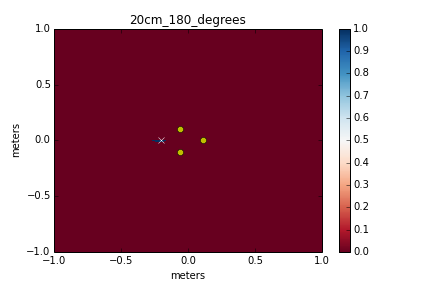
\includegraphics[width=\textwidth]{sim/result_20cm_180_degrees}
%    \caption{180 degrees}
%  \end{subfigure}
  \caption{Uncertainty region. Microphones are at the vertices of a $20$cm equilateral triangle. The source is $20$cm away from the array.}
  \label{fig:sim_3_2}
\end{figure*}

\begin{figure*}[]
  \centering
  \begin{subfigure}[]{.48\textwidth}
    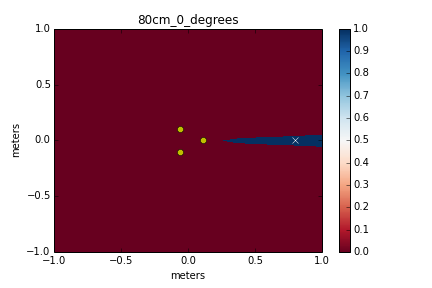
\includegraphics[width=\textwidth]{sim/result_80cm_0_degrees}
    \caption{0 degrees}
  \end{subfigure}
%  \begin{subfigure}[]{.3\textwidth}
%    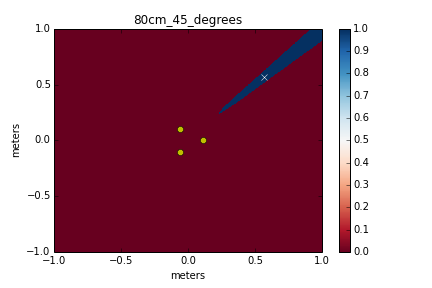
\includegraphics[width=\textwidth]{sim/result_80cm_45_degrees}
%    \caption{45 degrees}
%  \end{subfigure}
%  \begin{subfigure}[]{.3\textwidth}
%    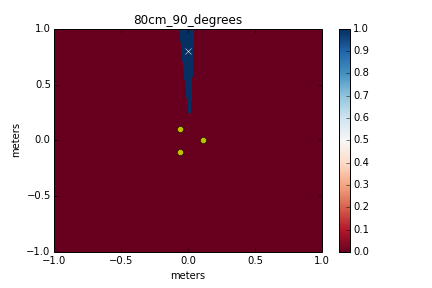
\includegraphics[width=\textwidth]{sim/result_80cm_90_degrees}
%    \caption{90 degrees}
%  \end{subfigure}
  \begin{subfigure}[]{.48\textwidth}
    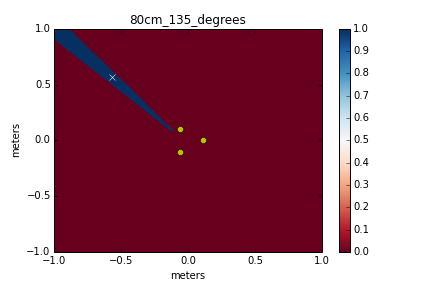
\includegraphics[width=\textwidth]{sim/result_80cm_135_degrees}
    \caption{135 degrees}
  \end{subfigure}
%  \begin{subfigure}[]{.3\textwidth}
%    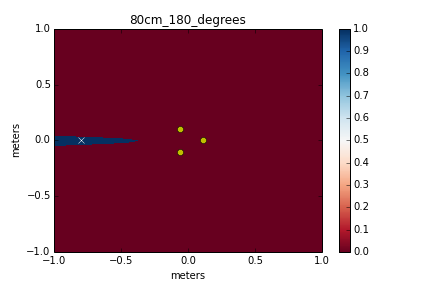
\includegraphics[width=\textwidth]{sim/result_80cm_180_degrees}
%    \caption{180 degrees}
%  \end{subfigure}
  \caption{Uncertainty region. Microphones are at the vertices of a $20$cm equilateral triangle. The source is $80$cm away from the array.}
  \label{fig:sim_3_8}
\end{figure*}

\section{Three Microphone Array}
With more than two microphones, each pair of microphones generates a hyperbolic region and localization becomes finding the intersection of hyperbolic regions. The smaller the intersection region, the better the localization accuracy. To see how accuracy changes with array placement and sound source location, three microphones are placed at the three vertices of a $20$ cm equilateral triangle. An audio source is placed at $20$ cm away from the center of the array. Fig~\ref{fig:sim_3_2} shows the intersection of regions for $2$ different placement of the sound source. It can be seen that accuracy decreases when sound source becomes close to the line connecting any two microphones. This observation is consistent with the two microphone case, since points close to lines connecting microphones have a larger uncertainty region.

To see how sound source distance affects localization accuracy, the same simulation is carried out with the sound source moved from $20$ cm to $80$ cm away from the center of the array. Results are presented in fig~\ref{fig:sim_3_8}. Comparing with fig~\ref{fig:sim_3_2}, accuracy decreases as the distance to the array increases. This is also consistent with our observation in $2$ microphone case where sources farther away would result in larger uncertainty region.

Each microphone pair generates a hyperbolic region, and the source location is in the intersection of these regions. The area of the intersection region is a measure of the localization accuracy: the smaller the area, the more certain we are about the source location. Different array configuration gives different intersection area size. To evaluate an array's accuracy in a region, we can place sound source at predetermined grid points in the region and look at the size of the intersection area for each tested point in the grid. The smaller the intersection area size, the better the configuration. Another measure we can use to evaluate an array configuration is the error distance between the centre of the intersection area to the actual source location. The smaller the error difference on average, the better the configuration. We used both the intersection area size and error distance as measures for evaluating the following configurations.
 
\subsection{Linear Configuration}

\begin{figure}[h!]
  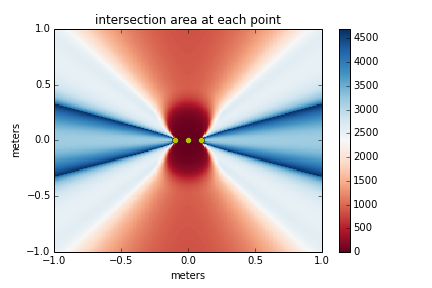
\includegraphics[width=\textwidth]{sim/result_intersection_area_at_each_point_3_line}
  \caption{Error heatmap for different array configurations. The heatmap scale is the intersection area measured in $cm^2$. $3$ microphones are placed in a line, $10$ cm apart from each other. The average error is $55.05$ cm}
  \label{fig:sim_hm_3_line}
\end{figure}


In fig~\ref{fig:sim_hm_3_line}, we experimented with an extreme arrangement where all three microphones are placed on a line, $10$ cm apart from each other. Looking at the figure above, we see that the intersection area is greater than $3000 \mathrm{cm}^2$ for points along the x axis. The average error distance is $55.05$ cm, which is not accurate enough for sub-meter localization. 

\subsection{Equilateral Triangular Configuration}

\begin{figure*}[h!]
\centering
  \begin{subfigure}[]{.48\textwidth}
    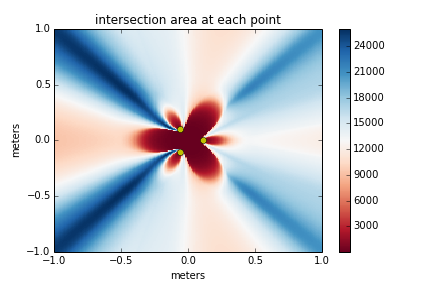
\includegraphics[width=\textwidth]{sim/result_intersection_area_at_each_point_3_center}
    \caption{$3$ microphones are placed at vertices of a $20$cm equilateral triangle. The average error is $18.6$ cm}
    \label{fig:sim_hm_3}
  \end{subfigure}
  \begin{subfigure}[]{.48\textwidth}
    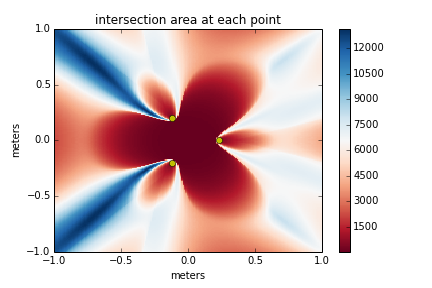
\includegraphics[width=\textwidth]{sim/result_intersection_area_at_each_point_3_2x}
    \caption{$3$ microphones are placed at vertices of a $40$cm equilateral triangle. The average error is $10.04$ cm}
    \label{fig:sim_hm_3_2x}
  \end{subfigure}
  \caption{Error heatmap for different array configurations. The heatmap scale is the intersection area measured in $cm^2$}.
\end{figure*}

Fig~\ref{fig:sim_hm_3} shows the accuracy when microphones are placed at the three vertices of a $20$ cm equilateral triangle. The region inside the array has good accuracy. However, for regions along the line connecting any two microphones, the accuracy drops significantly. The average distance error across the region is $18.6$ cm.

To evaluate the array size's impact on accuracy, the size of the original array (as in fig~\ref{fig:sim_hm_3}) is increased by a factor of $2$. The result is presented in fig~\ref{fig:sim_hm_3_2x}. The overall uncertainty area decreased across the region. The average error distance improved to $10.04$ cm. By comparing with the previous result, it shows that increasing array size is effective in improving the overall accuracy. 

\section{More than three}

\begin{figure*}[h!]
  \centering
  \begin{subfigure}[]{.48\textwidth}
    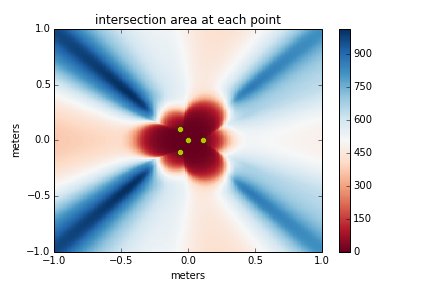
\includegraphics[width=\textwidth]{sim/result_intersection_area_at_each_point_3_p1}
    \caption{Another microphone is added at origin. The average error is $17.1$ cm}
    \label{fig:sim_hm_3_p1}
  \end{subfigure}
  \begin{subfigure}[]{.48\textwidth}
    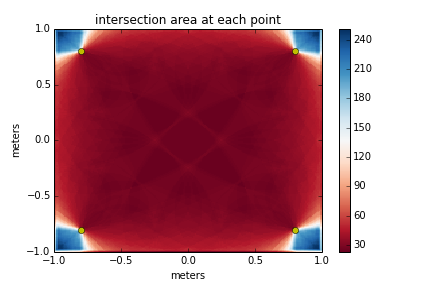
\includegraphics[width=\textwidth]{sim/result_intersection_area_at_each_point_4corner}
    \caption{$4$ microphones are placed at $4$ corners of the grid. The average error is $0.05$ cm}
    \label{fig:sim_hm_4}
  \end{subfigure}
  \begin{subfigure}[]{.48\textwidth}
    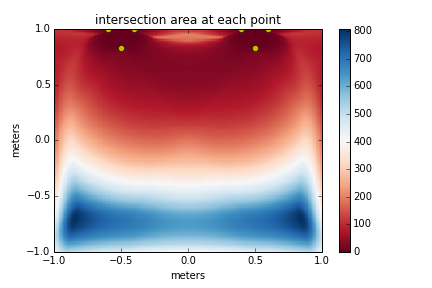
\includegraphics[width=\textwidth]{sim/result_intersection_area_at_each_point_2a}
    \caption{Two $3$ microphone arrays are placed $1$ meter apart. The average error is $2.60$ cm}
    \label{fig:sim_hm_2_array}
  \end{subfigure}
  \caption{Error heatmap for different array configurations. The heatmap scale is the intersection area measured in $cm^2$}.
\end{figure*}

To evaluate how adding one microphone (without increasing the array size) improves accuracy, another microphone is added at $(0,0)$ for the array described in fig~\ref{fig:sim_hm_3}. Result is presented in fig~\ref{fig:sim_hm_3_p1}. Addition of the new microphone only slightly improved the accuracy around the array region. The average distance error dropped from $18.6$ cm to $17.1$ cm. Regions near lines connecting microphones still have significantly large intersection area. This result suggests that adding more microphones in a small microphone array (without increasing the array size) is not an effective method for improving the localization accuracy.

To further increase the distance between microphones, we placed four microphones at four corners of the region. Fig~\ref{fig:sim_hm_4} shows the result. With this configuration, accuracy is consistently good across the region. The average distance error is $0.05$ cm.  However, placing microphones far apart at corners of the region requires accurate placement of all four individual microphones. The system is less portable compared to small arrays with microphones near each other. Placing microphones far apart from each other also causes problems in TDOA estimation, because sampling of microphones in the same array requires synchronized clock.

To avoid the need to accurately place microphones at far distances (as required by fig~\ref{fig:sim_hm_4}), we explored configuration with two arrays. Two $3$ microphone array are placed $1$ meter apart and the result is presented in fig~\ref{fig:sim_hm_2_array}.  The result indicates that this configuration has good accuracy when source is close to the arrays. We observe that the localization accuracy decreases as the sound source moves outside of the one meter by one meter region away from the two arrays. The average error is $2.60$ cm. In general, synchronized clocks must be used to sample microphone data to ensure accurate comparison of arrival time differences. In practice, this means clocks must be synchronized for all the microphones across the two arrays. In the next chapter, we will describe a method that does not require clocks to be synchronized across the two arrays. This approach would make the system easier to design, although clocks still needs to be synchronized for microphones within the same array. 


\section{Discussion}

Looking at the simulation results on localization accuracy for different microphone array size and configurations, we see that the further away the microphones are placed from each other the higher the localization accuracy. However, as we increase the distance between each microphone pairs, the size of the overall array increases and the system becomes less portable. In the end we decided to build the two array system as described in fig~\ref{fig:sim_hm_2_array}. The setup is reasonably portable (compared to fig~\ref{fig:sim_hm_4}), yet it can achieve on average high localization accuracy within a region one meter by one meter close the setup. Since our target application is HCI, an one meter by one meter region will be adequate for this purpose and it will be used for all the following experiments.   
